\chapter{Static Analysis Tools}

% TODO: might be worth talking about soundness and completeness

Static program analysis is the process of automatically analysing source code to extract information about its behavior without executing it, as opposed to dynamic analysis, which is performed on programs as they are run.
Static analysis tools can ease the burden of software development by automating tasks that would otherwise require manual effort and meticulous attention to detail.
These tools can perform a variety of tasks, ranging from detecting possible bugs \cite{johnson_lint_1978,hovemeyer_finding-bugs_2004} to formal software verification of program properties \cite{blanchet_static-analyzer_2003}.

Static analysis tools are increasingly becoming more important in modern software development, as modern code continues to become more complex and difficult to reason about.
Industry leaders, such as Google \cite{sadowski_analysis-google_2018} and Meta (formerly Facebook) \cite{calcagno_moving-facebook_2015}, have embraced static analysis tools as integral components of their software development workflows.

\section{Applications of Static Analysis Tools}
Typically in a software development workflow, multiple static analysis tools are used in conjunction to provide a comprehensive suite of checks.
Often, these tools are integrated into an \textsc{ide} as plugins, allowing them to be consolidated into a single visual interface.

% TODO: is this paragraph now a bit off-topic compared to what is actually discussed?
Refactoring and linting are two major functionalities that these tools provide.
However, because many of these tools include both capabilities, the distinction between them can be blurry.
This section aims to establish definitions for the two terms, which will be used as a basis for subsequent discussion within this thesis.

\subsection{Automated Refactoring}
Code refactoring is a well-established practice in software development.
In his influential book \textit{Refactoring: Improving the Design of Existing Code} \cite{fowler_refactoring_2018}, Fowler defines \textbf{refactoring} as ``the process of changing a software system in such a way that it does not alter the external behavior of the code yet improves its internal structure''.
Refactoring may be employed to eliminate \textbf{code smells}, which are surface indications that could indicate deeper problems in the system.
Code smells are not necessarily problematic on their own, however, they may lead to issues such as bugs or poor maintainability if left unchecked.
Examples of code smells include duplicated code, which can be hard to update without introducing bugs, and long methods, which can be difficult to understand and maintain.
Therefore, it is often productive to refactor code to eliminate code smells, even if the code is still correct and functional.

Static analysis tools can reason about how to safely refactor code in an automated manner, performing refactorings as source-to-source transformations.
These transformations may be implemented as simple text-based replacements or more robust rewrite rules that operate on the abstract syntax tree (\textsc{ast}) of the source code.

Automated refactoring support is particularly useful for large codebases, where manual refactoring would be tedious and error-prone.
Generally, when a user makes use of an automated refactoring tool in an \textsc{ide}, they will manually identify the snippet of code that they wish to refactor, and then select the appropriate refactoring from a list of available options.
Fig.~\ref{fig:extract-function-intellij} presents \textit{Extract Method} \cite{fowler_refactoring_2018} in the IntelliJ IDEA\footnote{\url{https://www.jetbrains.com/idea/}} \textsc{ide}, an example of a common refactoring that can be performed automatically on a block code selected by the user.

\begin{figure}[htbp]
  \centering
  \begin{subfigure}{\textwidth}
    \centering
    \begin{minted}[frame=single,highlightlines={4-5},linenos]{scala}
      object Main {
        def main(args: Array[String]): Unit = {
          val bankDetails = getBankDetails()
          println(s"Account name: ${bankDetails.name}")
          println(s"Account balance: ${bankDetails.balance}")
        }
      }
    \end{minted}
    \caption{A snippet of Scala code. A user may wish to extract the highlighted lines into a separate function.}
    \label{fig:extract-function-intellij-before}
  \end{subfigure}
  \begin{subfigure}{\textwidth}
    \centering
    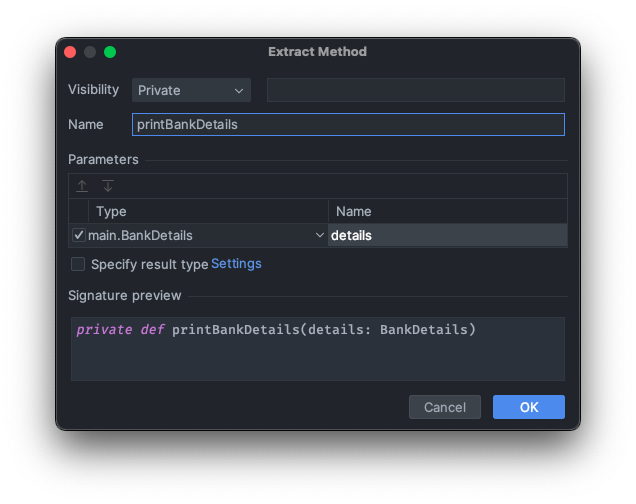
\includegraphics[width=0.75\textwidth]{background/extract-function-intellij.png}
    \caption{When a user selects the highlighted lines from fig.~\ref{fig:extract-function-intellij-before} in IntelliJ IDEA, choosing the \textit{Extract Method} refactoring will open this dialogue to preview changes before applying them.}
    \label{fig:extract-function-intellij-dialogue}
  \end{subfigure}
  \begin{subfigure}{\textwidth}
    \vspace{3ex} % TODO: ew
    \centering
    \begin{minted}[frame=single,highlightlines={4,7-10},linenos]{scala}
      object Main {
        def main(args: Array[String]): Unit = {
          val bankDetails = getBankDetails()
          printBankDetails(bankDetails)
        }

        private def printBankDetails(details: BankDetails): Unit = {
          println(s"Account name: ${details.name}")
          println(s"Account balance: ${details.balance}")
        }
      }
    \end{minted}
    \caption{The result of applying the \textit{Extract Method} refactoring using the chosen parameters in fig.~\ref{fig:extract-function-intellij-dialogue}.}
  \end{subfigure}
  \caption{An example of the \textit{Extract Method} refactoring in IntelliJ IDEA.}
  \label{fig:extract-function-intellij}
\end{figure}

\subsection{Linting}
\textbf{Linting} is the process of analysing source code to identify and report issues related to coding style and potential logical errors.
The term originates from the \texttt{lint} program \cite{johnson_lint_1978}, which examined C source code for bugs, as well as wasteful code patterns that may be legal but error-prone.
The tool was also utilised to enforce portability restrictions which aided users in writing portable code that could be compiled on multiple platforms.
Since the release of \texttt{lint}, many linting tools, known as \textbf{linters}, have been developed for a wide range of programming languages.

Linters are provided as standalone tools separate from a compiler, since their primary goal is to suggest improvements for code readability and maintainability, rather than code optimisations.
Modern linters are commonly integrated into \textsc{ide}s, where code analysis performed by the linter is run incrementally in the background.
Any violations found by the linter are displayed directly in the editor as warnings or errors at the relevant locations in the source code.
This provides an ergonomic user experience, as the user can see the results of the analysis in real-time as part of the development workflow.

Although the strict definition for linting is concerned with only detecting issues in code, many advanced linters today can also provide auto-fixes for violations which can be corrected automatically by static analysis.
This auto-fix capability is often integrated into \textsc{ide}s as well: the popular Language Server Protocol for defining \textsc{ide} features enables these auto-fix features via \textit{code actions} \cite{gunasinghe_lsp_2022}.
When a section of code is highlighted by a linter warning, a user can apply a code action to automatically fix the issue with a single click.

Many linters are configurable with a set of rules, which specify the types of issues that the linter should detect.
These rules can be enabled or disabled by the user, allowing them to customise the linter to their needs.
Rules can be categorised by their purpose: some rules are concerned with enforcing code style, while others are concerned with detecting code smells or other suspicious code patterns indicative of possible bugs.

\subsubsection{Style checking and code appearance}
% TODO: CheckStyle https://checkstyle.sourceforge.io/?
Linters can be configured to enforce a particular style guide defining a set of conventions for how idiomatic code should be written.
They can highlight style violations and in basic cases, automatically rewrite code to conform to the correct style.
For example, the \textit{Flake8}\footnote{\url{https://flake8.pycqa.org/en/latest/}} linter for Python enforces coding conventions from the PEP 8 style guide \cite{van_rossum_pep8_2001}.
Stylistic rules are especially helpful for large projects with multiple contributors, where a consistent coding style can improve readability and maintainability.

\subsubsection{Identifying opportunities for refactoring}
Certain linting rules can aid in the refactoring process by broadly identifying code smells and candidate areas for refactoring, suggesting appropriate actions that the user can take.
As an example, a linter may detect a fragment of code that is repeated in multiple places: this is a code smell, as discussed previously.
The linter may then suggest a code action to automatically apply the \textit{Extract Method} refactoring to avoid code duplication.

\subsubsection{Suggesting idiomatic usage}
Other rules can suggest opportunities to improve more precise snippets of code by utilising language features in a more idiomatic manner.
These rules are especially helpful for new users of a language, who may be unaware of useful language constructs and idioms.
For example, the \textit{Clippy}\footnote{\url{https://doc.rust-lang.org/clippy/}} linter for Rust \cite{li_clippy_2023} categorises a collection of rules as \texttt{clippy::complexity} rules to detect code that does something simple in a complex way and suggests a simpler alternative.
Fig.~\ref{fig:hlint-example} provides an example of a similar rule in Haskell, from the \textit{HLint}\footnote{\url{https://hackage.haskell.org/package/hlint}} linter.
The rule suggests an $\eta$-reduction refactoring, presented to the user as a code action that can be applied automatically.

\begin{figure}[htbp]
  \vspace{3ex} % TODO: make this less hacky
  \centering
  \begin{subfigure}{0.45\textwidth}
    \centering
    \begin{minted}[frame=single]{haskell}
      foo xs = map (+1) xs
    \end{minted}
    \caption{A Haskell function \texttt{foo}, which can be made more concise using $\eta$-reduction.}
  \end{subfigure}
  \hfill
  \begin{subfigure}{0.45\textwidth}
    \centering
    \begin{minted}[frame=single,escapeinside=||]{text}
      Eta reduce
      Found:
        foo xs = map (+ 1) xs
      Why not:
        foo = map (+ 1)
      |\textcolor{gray}{hlint(refact:Eta reduce)}|
    \end{minted}
    \caption{The linter warning shown for \texttt{foo}.}
  \end{subfigure}
  \caption{An example of a warning from the Haskell linter \texttt{hlint}, suggesting a fix that a user can choose to automatically apply.}
  \label{fig:hlint-example}
\end{figure}

Many idiomatic practices exist to avoid common pitfalls that may lead to unintended behaviour.
By highlighting good practices, linters can help users avoid these common mistakes that may cause bugs.
For example, \textit{ESLint}\footnote{\url{https://eslint.org/docs/latest/rules/}}, one of the most popular JavaScript linters, warns against common JavaScript pitfalls such as using the regular equality operator \texttt{==} instead of its type-safe alternative \texttt{===}.

Linters developed for a specific library provide rules to enforce idiomatic usage specific to the domain of the library.
A library or especially an embedded \textsc{dsl} may require a particular style of usage that is different from the host language \cite{hora_domain_2012}.
Therefore, a regular linter for the host language may not be able to detect issues specific to the library.
In this case, an accompanying linter can greatly benefit users: common misuses can be detected and sometimes automatically fixed, and users can be directed to relevant documentation to learn more about correct usage.
For instance, the \textit{xUnit.net} testing framework for C\# is accompanied by the \texttt{xunit.analyzers}\footnote{\url{https://github.com/xunit/xunit.analyzers}} package which provides linting rules to enforce best practices specific to xUnit.

\subsubsection{Detecting potential bugs}
Linters may also directly attempt to detect more serious issues in code, such as possible logic errors.
This can be helpful for even experienced users to avoid common pitfalls.
Clippy has \texttt{clippy::suspicious} and \texttt{clippy::correctness} rule categories to identify code that is very likely to be incorrect or useless.
ESLint provides several rules to warn against code patterns that are likely to cause runtime errors, such as re-assigning a \texttt{const} variable.

\section{Static Analysis for Scala}
\subsection{Choice of Tooling}
The goal of \texttt{parsley-garnish} is to provide linting and refactoring capabilities for the \texttt{parsley} parser combinator library.
Since \texttt{parsley} is a Scala library, this project must be implemented using a tool capable of statically analysing Scala code.
This section will therefore discuss and evaluate the choices available for implementing \texttt{parsley-garnish}.

\subsubsection{Scala compiler plugins}
The most powerful approach would be to implement \texttt{parsley-garnish} as a compiler plugin \cite{pickering_plugins_2019}.
Using the low-level compiler \textsc{api}, it is possible to perform arbitrary code transformations at any step of the compilation process.
Compiler plugins therefore offer full freedom to extend the Scala compiler with extra functionality, such as extra passes for code analysis and emitting lint warnings as diagnostics or even compiler errors.

However, this approach has several drawbacks.
Firstly, compiler plugins are tightly coupled with the compiler itself, and therefore not portable across major compiler versions.
% https://github.com/mattmoore/scala-compiler-plugins is a good reference, in case I need to revisit this
For instance, plugins written for the Scala 3 compiler, known as \texttt{dotty}, are completely incompatible with Scala 2 plugins \cite{lampepfl_changes_2022}.
Additionally, developing compiler plugins requires a deep understanding of arcane and poorly documented compiler internals.
Exposing the full compiler \textsc{api} permits unsafe operations that may violate undocumented invariants assumed by the compiler, leading to exceptions during compilation or even malformed bytecode \cite{sherwany_refactoring_2015}.
The lack of higher-level abstractions also makes it difficult to implement even trivial tasks such as renaming a field.

For these reasons, it would be preferable to explore other tools that may use compiler plugins themselves but provide a higher-level interface for implementing code analysis and transformations.

\subsubsection{Scalameta}
\textit{Scalameta}\footnote{\url{https://scalameta.org/}} is a metaprogramming framework for Scala that provides a unified interface for performing common metaprogramming tasks.
It provides a high-level syntactic \textsc{api} for transforming and pretty-printing Scala source code, as well as a semantic \textsc{api} providing access to semantic information such as type inference and name resolution.
Scalameta is the successor of the earlier \texttt{scala.reflect} metaprogramming framework, which parsed source code into lossy trees that discarded syntactic information such as comments and whitespace \cite{burmako_scalameta_2017}.
On the other hand, Scalameta trees are lossless and preserve all syntactic details, a key feature that allows code transformations and refactorings to preserve formatting details.

Scalameta's semantic \textsc{api} is powered by \textit{SemanticDB}, a compiler-agnostic data model for semantic information in Scala programs.
This allows Scalameta to extract semantic information via compiler plugins that emit data in the SemanticDB format.
Thus, Scalameta can work with any compiler that supports SemanticDB, rather than being tied to a specific compiler implementation.

Since Scalameta provides a high-level interface for manipulating syntactic and semantic information, it is a promising choice for this project.
Being able to access semantic information is especially helpful for implementing more complex code analyses.
However, Scalameta's primary focus is on providing a general metaprogramming framework and therefore lacks \textsc{api} support specifically for implementing linting and refactoring rules.
For example, the Scalameta tree transformation utilities do not preserve formatting details when pretty-printed, despite the underlying trees containing this information.

\subsubsection{Scalafix}
\textit{Scalafix}\footnote{\url{https://scalacenter.github.io/scalafix/}} is a refactoring and linting tool built on top of Scalameta.
It specifically provides an \textsc{api} for implementing fine-grained code transformations that preserve comments and formatting details.
Scalafix provides a framework for implementing linting rules to emit warnings, as well as rewrite rules to perform automated code transformations \cite{geirsson_catch_2017}.
Since it is built on Scalameta, a major advantage of Scalafix is that it is also compiler-agnostic and could be integrated into any \textsc{ide} if a plugin is developed for it.

Originally, Scalafix was designed to help automate the process of migrating code from Scala 2 to 3, which involved many breaking changes to the language \cite{geirsson_scalafix_2016}.
However, Scalafix has since evolved into a general-purpose tool for implementing code transformations and analyses, utilising the powerful syntactic and semantic \textsc{api}s provided by Scalameta.
Scalafix rules can be either syntactic or semantic, depending on whether they require semantic information to perform their analysis.
Syntactic rules are faster to run, since they operate purely on the \textsc{ast} without requiring compilation to extract semantic information, but are more limited in the accuracy of analyses they can perform.

Scalafix is growing to become the de-facto modern successor to earlier refactoring tools such as Abide\footnote{\url{https://contributors.scala-lang.org/t/whats-the-status-of-abide/}} and \texttt{scala-refactoring}\footnote{\url{https://github.com/scala-ide/scala-refactoring}}.
\texttt{scala-refactoring} used \texttt{scala.reflect} to implement code transformations, with much extra work utilising the Scala Presentation Compiler \textsc{ast} to preserve formatting details lost by \texttt{scala.reflect}.
As a result, maintaining the library became difficult and the project was abandoned in favour of a clean implementation using Scalameta, which was designed in part to address the shortcomings of \texttt{scala.reflect}.

A drawback of Scalafix is that it is primarily a command-line tool, and therefore by default does not provide a user-friendly interface for interactive usage.
However, this can rectified in the future by integrating Scalafix into the Metals \textsc{lsp} server for Scala, which would allow it to be integrated into any \textsc{ide} that supports the LSP.

Overall, Scalafix emerges as the most favorable choice for implementing \texttt{parsley-garnish}.
It provides high-level \textsc{api}s specifically for implementing linting and rewrite rules without necessitating extensive knowledge of compiler internals.
Scalafix is also being actively developed and maintained, with good basic documentation and a growing number of examples of usage in the wild.

\subsubsection{Other tools considered}
The main alternate contender to Scalafix is the IntelliJ Scala Plugin\footnote{\url{https://github.com/JetBrains/intellij-scala}}.
However, while the plugin offers superior interactive usage within the IntelliJ IDEA \textsc{ide}, it is tied to the IntelliJ Scala compiler and therefore not portable across other compilers.
To maintain flexibility and not tie \texttt{parsley-garnish} to a particular compiler or code editor, Scalafix is a preferable option.
Furthermore, documentation is less clear on how to write a Scala plugin for IntelliJ compared to the Scalafix documentation.

WartRemover\footnote{\url{https://www.wartremover.org/}} is a linter implemented as a compiler plugin, with support for writing custom rules.
However, it only can emit warnings or errors and does not support auto-fixes, making it less suitable for \texttt{parsley-garnish}'s goals.

ScalaStyle\footnote{\url{http://www.scalastyle.org/}} is primarily a style checker which also supports custom rules.
However, it is only able to perform syntactic analyses and does not have access to semantic information, restricting the types of analyses it can perform.

% TODO: maybe a section introducing ScalaFix and how it works? or is that too much detail?
% TODO: maybe a figure to show an example of a ScalaFix rewrite rule?

% TODO: comparison with clippy (https://doc.rust-lang.org/clippy/development/lint_passes.html) and/or roslyn (https://learn.microsoft.com/en-us/dotnet/csharp/roslyn-sdk/; https://learning.oreilly.com/library/view/roslyn-cookbook/9781787286832/)
